\documentclass[12pt]{article}
\usepackage{graphicx,multicol,mdwlist}
\usepackage{charter,amsmath,amssymb,breakurl}
\usepackage{eulervm}
\usepackage[letterpaper,margin=1in]{geometry}
\title{Math 265 Quiz 3 Warmup}\author{}\date{}
\let\cos\relax\DeclareMathOperator{\cos}{\mathsf{cos}}
\let\ln\relax\DeclareMathOperator{\ln}{\mathsf{ln}}
\everymath{\displaystyle}
\begin{document}
\maketitle
\thispagestyle{empty}
\begin{multicols}{2}
Questions~\ref{FirstEllipse}--\ref{LastEllipse}
deal with the vector field $\mathbold{F}\left(x,y\right)
=\left\langle x^2-y^2,xy\right\rangle$, which is shown
at the right, together with the curve $C$ consisting of
the top arc of the ellipse $x^2+\frac{y^2}{4}=1$
joined with the line segment from $\left(-1,0\right)$
to $\left(0,1\right)$.
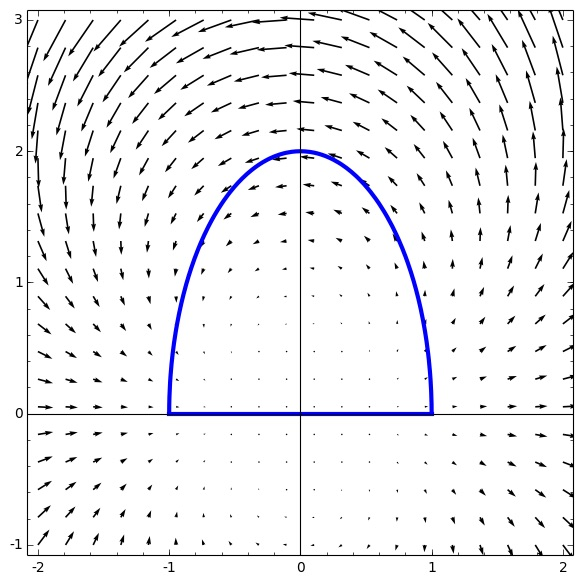
\includegraphics[scale=.4]{Ellipse}
\end{multicols}
\begin{enumerate}
\item\label{FirstEllipse}
Calculate the circulation $\oint_C\mathbold{F}
\cdot d\mathbold{r}$ directly.
\item Calculate the circulation $\oint_C\mathbold{F}
\cdot d\mathbold{r}$ using Green's Theorem.
\item\label{LastEllipse} Calculate the outward flux $\oint_C\mathbold{F}
\cdot\mathbold{n}\;ds$ using Green's Theorem.
\suspend{enumerate}
Questions~\ref{FirstConservative}--\ref{LastConservative}
deal with
the vector field $\mathbold{F}\left(x,y,z\right)
=\left\langle 2xy+z^2,x^2,2xz\right\rangle$
and the circle $C$ given by
\[\mathbold{r}\left(t\right)=\left\langle
3\cos{t},4\cos{t},5\sin{t}\right\rangle\]
with $0\le t\le 2\pi$.
\resume{enumerate}
\item\label{FirstConservative} Is $\mathbold{F}$ conservative?
\item Calculate the circulation $\oint_C\mathbold{F}
\cdot d\mathbold{r}$ using a method of your choice.
\item\label{LastConservative}
Calculate the line integral $\int_D\mathbold{F}
\cdot d\mathbold{r}$ using a method of your choice,
where $D$ is the arc of $C$ with $0\le t\le\frac{\pi}{2}$.
\end{enumerate}
\end{document}
